\documentclass{article}
\usepackage{graphicx}
\usepackage{subcaption}
\usepackage{xcolor}
\usepackage{tikz}

\begin{document}

\begin{figure*}[t]
\centering

% Subfigura a) - Aumentada
\begin{subfigure}[b]{0.58\textwidth}
    \centering
    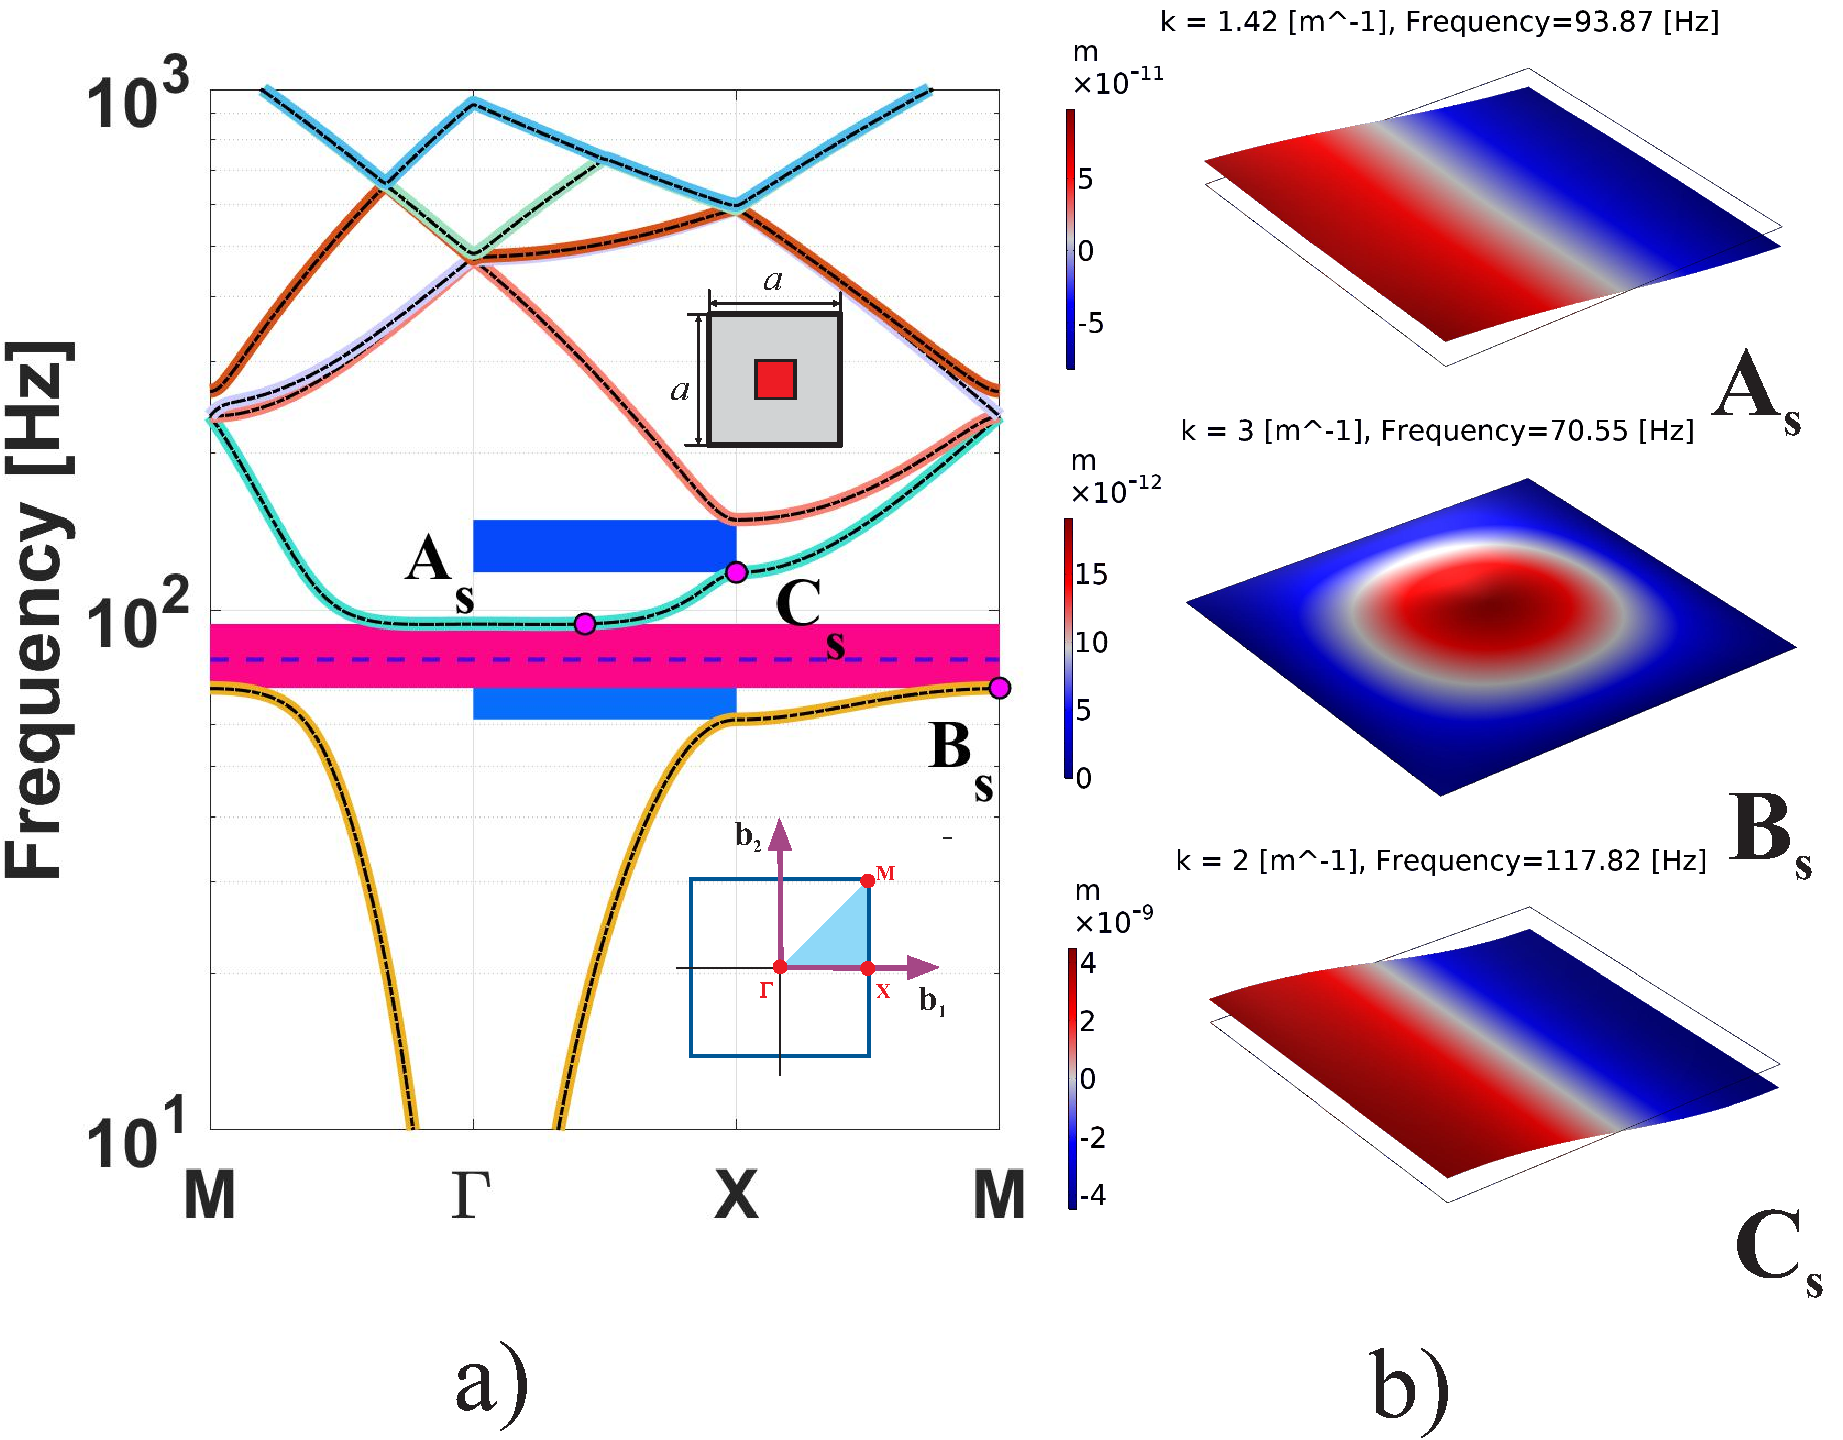
\includegraphics[width=\textwidth]{1_1_disp_frf_square.pdf}
    \caption{Dispersion diagram}
    \label{fig:dispersion_square}
\end{subfigure}
\hfill
% Subfigura b) - Aumentada
\begin{subfigure}[b]{0.38\textwidth}
    \centering
    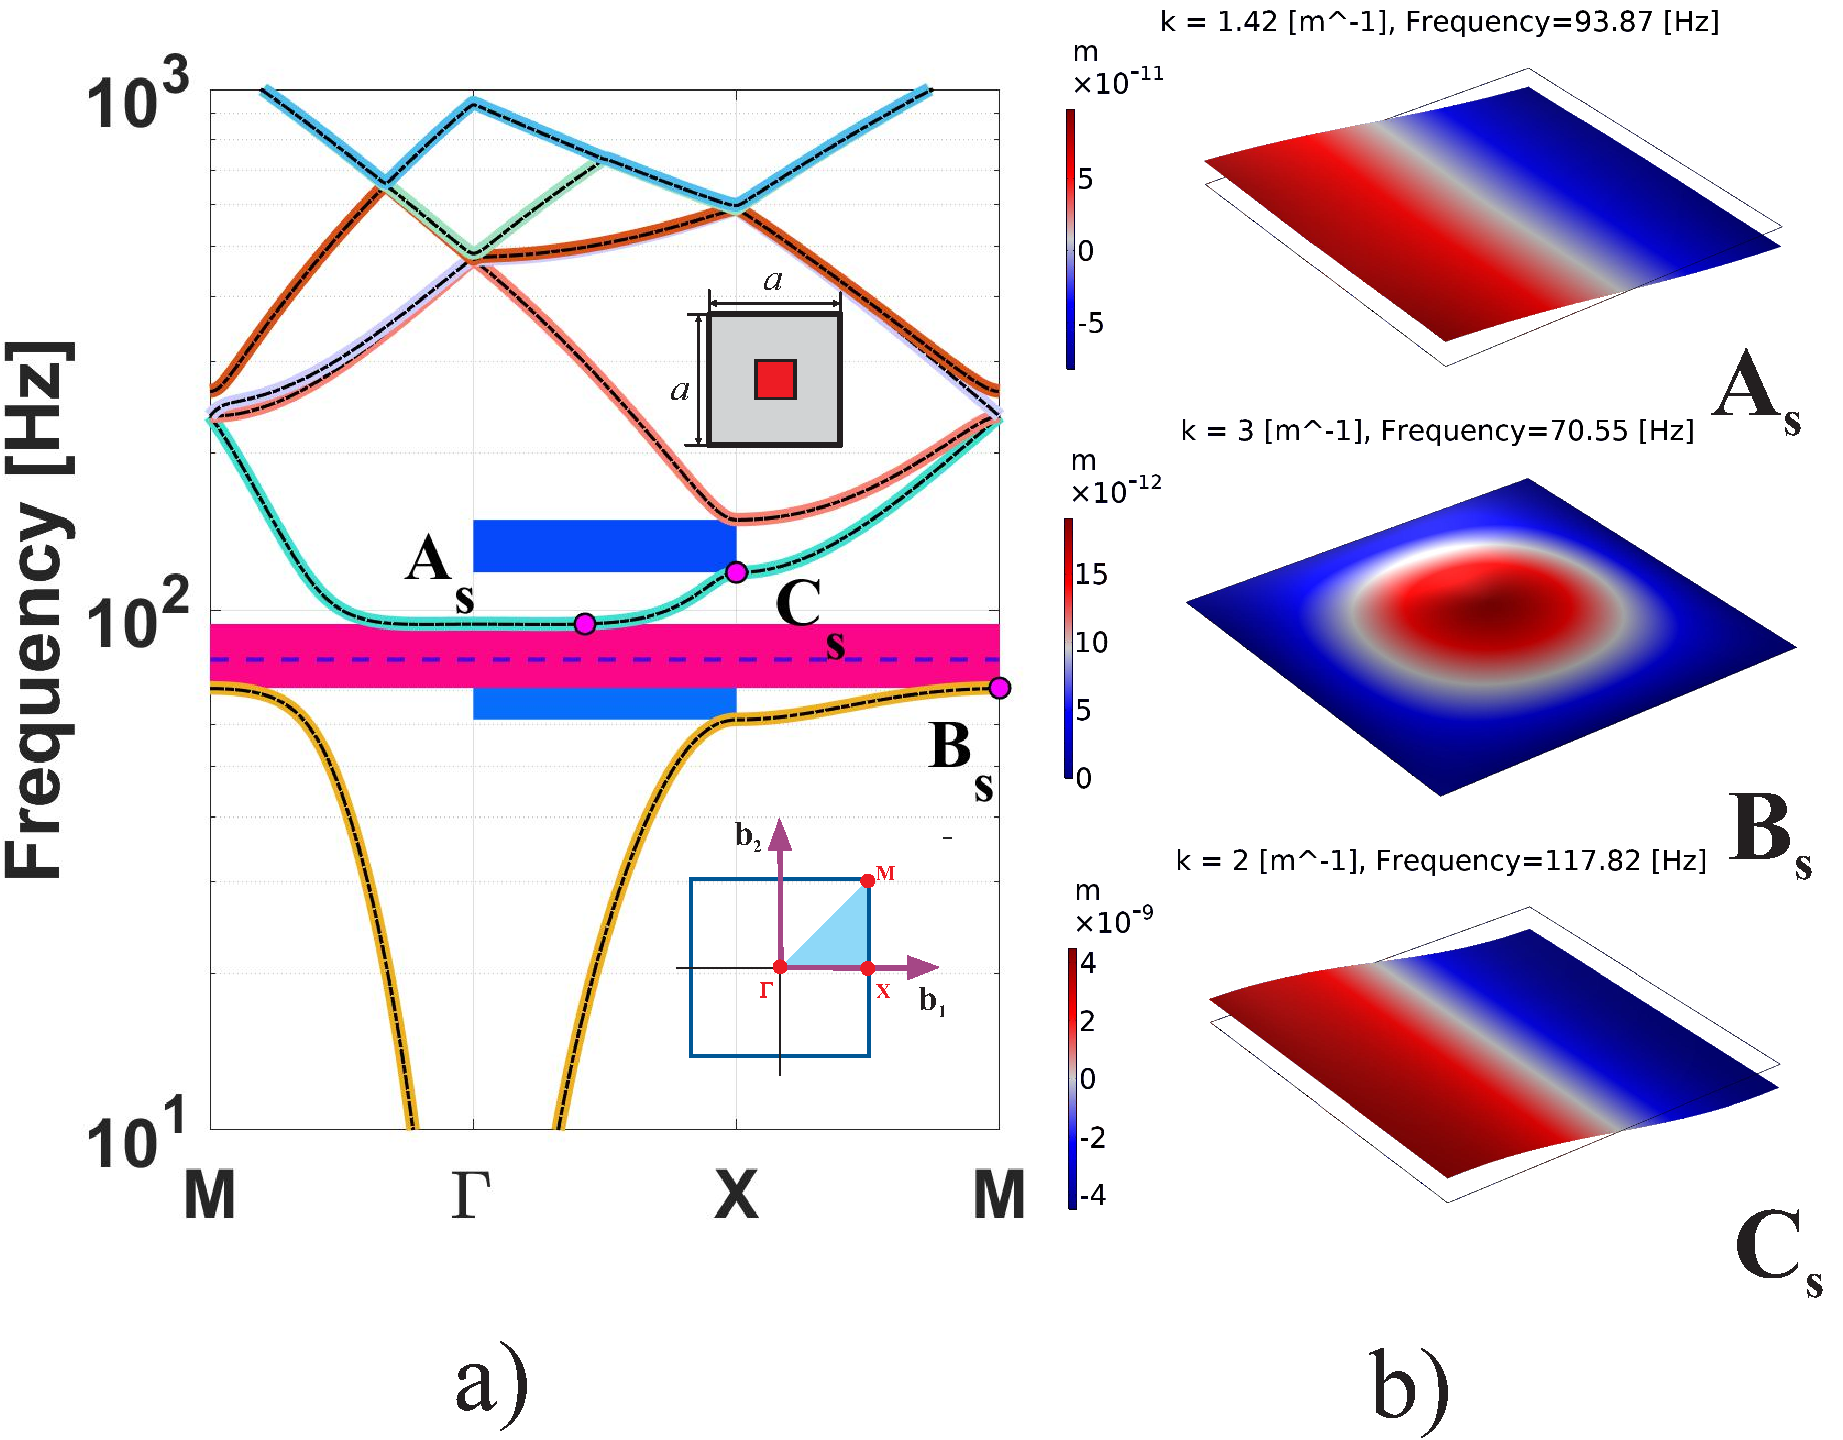
\includegraphics[width=\textwidth]{1_1_disp_frf_square.pdf}
    \caption{Wave modes}
    \label{fig:wavemodes_square}
\end{subfigure}

\vspace{0.3cm}

% Legenda externa em LaTeX com informações numéricas
\scriptsize
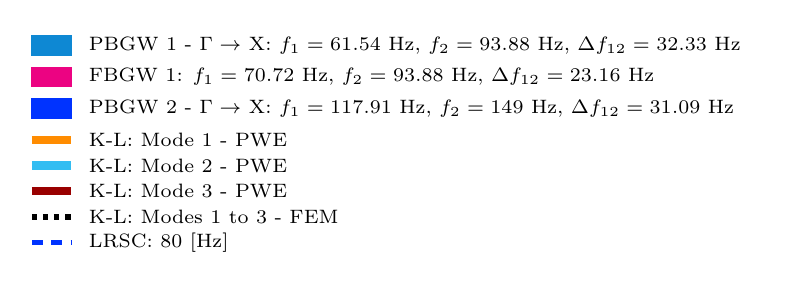
\begin{tikzpicture}[scale=1.0]
    % Linha 1 - PBGW 1 (RETÂNGULO azul claro/ciano)
    \filldraw[cyan!70!blue] (0,0) rectangle (0.5,0.25);
    \node[right, font=\scriptsize, align=left] at (0.6,0.125) {
        PBGW 1 - $\Gamma \rightarrow$ X: $f_1 = 61.54$ Hz, $f_2 = 93.88$ Hz, $\Delta f_{12} = 32.33$ Hz
    };

    % Linha 2 - FBGW 1 (RETÂNGULO magenta)
    \filldraw[magenta!90!red] (0,-0.4) rectangle (0.5,-0.15);
    \node[right, font=\scriptsize, align=left] at (0.6,-0.275) {
        FBGW 1: $f_1 = 70.72$ Hz, $f_2 = 93.88$ Hz, $\Delta f_{12} = 23.16$ Hz
    };

    % Linha 3 - PBGW 2 (RETÂNGULO azul)
    \filldraw[blue!80!cyan] (0,-0.8) rectangle (0.5,-0.55);
    \node[right, font=\scriptsize, align=left] at (0.6,-0.675) {
        PBGW 2 - $\Gamma \rightarrow$ X: $f_1 = 117.91$ Hz, $f_2 = 149$ Hz, $\Delta f_{12} = 31.09$ Hz
    };

    % Linha 4 - K-L Mode 1 (LINHA laranja)
    \draw[line width=3pt, orange!90!yellow] (0,-1.075) -- (0.5,-1.075);
    \node[right, font=\scriptsize] at (0.6,-1.075) {K-L: Mode 1 - PWE};

    % Linha 5 - K-L Mode 2 (LINHA ciano claro)
    \draw[line width=3pt, cyan!80!white] (0,-1.4) -- (0.5,-1.4);
    \node[right, font=\scriptsize] at (0.6,-1.4) {K-L: Mode 2 - PWE};

    % Linha 6 - K-L Mode 3 (LINHA vermelho escuro)
    \draw[line width=3pt, red!60!black] (0,-1.725) -- (0.5,-1.725);
    \node[right, font=\scriptsize] at (0.6,-1.725) {K-L: Mode 3 - PWE};

    % Linha 7 - FEM (LINHA tracejada preta)
    \draw[line width=2pt, black, dash pattern=on 2pt off 2pt] (0,-2.05) -- (0.5,-2.05);
    \node[right, font=\scriptsize] at (0.6,-2.05) {K-L: Modes 1 to 3 - FEM};

    % Linha 8 - LRSC (LINHA tracejada azul)
    \draw[line width=2pt, blue!80!cyan, dash pattern=on 4pt off 3pt] (0,-2.375) -- (0.5,-2.375);
    \node[right, font=\scriptsize] at (0.6,-2.375) {LRSC: 80 [Hz]};
\end{tikzpicture}

\caption{Band structure and wave mode shapes for a square lattice unit cell with single resonator ($f_r = 80$ Hz) in a thin plate. (\textit{a}) Dispersion diagram computed with PWE and FEM methods along M--$\Gamma$--X--M showing FBGW 1 ($f_1 = 70.72$ Hz, $f_2 = 93.88$ Hz, $\Delta f_{12} = 23.16$ Hz), PBGW 1 ($\Gamma \rightarrow$ X: $f_1 = 61.54$ Hz, $f_2 = 93.88$ Hz, $\Delta f_{12} = 32.33$ Hz), and PBGW 2 ($\Gamma \rightarrow$ X: $f_1 = 117.91$ Hz, $f_2 = 149$ Hz, $\Delta f_{12} = 31.09$ Hz). (\textit{b}) Wave mode shapes at points $A_s$, $B_s$, and $C_s$ computed by FEM.}
\label{pwe_fem_disp_modal_square}
\end{figure*}

\end{document}
